\documentclass[aspectratio=169,10pt]{beamer}

% ============================================================
%  Curso de Maestría — Métodos de Optimización
%  Clase 1: Introducción y conceptos matemáticos básicos
% ============================================================

\usepackage[utf8]{inputenc}
\usepackage[T1]{fontenc}
\usepackage{lmodern}
\usepackage[spanish]{babel}
\usepackage{amsmath,amssymb,amsthm}
\usepackage{graphicx}
\usepackage{booktabs}
\usepackage{xcolor}
\usepackage{listings}
\usepackage{tikz}

\graphicspath{{figs/}}

\usetheme{metropolis}
\metroset{block=fill, progressbar=frametitle, sectionpage=progressbar, numbering=fraction}

\definecolor{pygreen}{RGB}{0,128,0}
\definecolor{pyblue}{RGB}{0,0,180}
\definecolor{pygray}{RGB}{110,110,110}
\definecolor{codebg}{RGB}{245,245,245}

\lstdefinestyle{pythonstyle}{
  language=Python,
  backgroundcolor=\color{codebg},
  basicstyle=\ttfamily\scriptsize,
  keywordstyle=\color{pyblue}\bfseries,
  commentstyle=\color{pygreen}\itshape,
  stringstyle=\color{pygray},
  numbers=none,
  breaklines=true,
  showstringspaces=false,
  frame=single,
  rulecolor=\color{gray!40},
  xleftmargin=4pt,
  xrightmargin=4pt,
  aboveskip=6pt,
  belowskip=2pt,
}
\lstset{style=pythonstyle}

% --- notación abreviada ---
\newcommand{\R}{\mathbb{R}}
\newcommand{\grad}{\nabla}
\newcommand{\x}{\mathbf{x}}
\newcommand{\dd}{\mathbf{d}}
\renewcommand{\u}{\mathbf{u}}
\newcommand{\Hess}{\nabla^2 f}

\title{Métodos de Optimización}
\subtitle{Clase 1: Introducción y conceptos matemáticos básicos}
\author{[Nombre del profesor]}
\institute{Programa de Maestría, [Nombre de la universidad / programa]}
\date{Septiembre de 2026}

\begin{document}

% ---------------------------------------------------------------
\begin{frame}[plain]
  \maketitle
\end{frame}

\begin{frame}{Contenido}
  \footnotesize
  \begin{columns}[T]
    \column{0.5\textwidth}
    \begin{enumerate}
      \setcounter{enumi}{0}
      \item ¿Qué es optimizar?
      \item Derivada de una función de una variable
      \item Funciones de varias variables y parciales
      \item El vector gradiente
      \item Curvas de nivel
      \item Derivada direccional y máx.\ crecimiento
      \item Monotonía
      \item Puntos críticos
      \item La matriz Hessiana
    \end{enumerate}
    \column{0.5\textwidth}
    \begin{enumerate}
      \setcounter{enumi}{9}
      \item Serie de Taylor
      \item Convexidad
      \item Máx./mín.\ locales vs.\ globales
      \item Optimización sin restricciones
      \item Restricciones de igualdad (Lagrange)
      \item Restricciones de desigualdad (KKT)
      \item Síntesis de la clase
      \item Ejercicios propuestos
      \item Referencias
    \end{enumerate}
  \end{columns}
\end{frame}

% ==================================================================
\section{¿Qué es optimizar?}
% ==================================================================

\begin{frame}{¿Qué es optimizar?}
  \begin{alertblock}{Idea clave}
    Optimizar es \textbf{elegir, entre muchas alternativas posibles, la mejor
    según un criterio numérico}: el menor costo, el mayor beneficio, el menor
    error, el menor tiempo, la mayor resistencia, etc.
  \end{alertblock}
  \vspace{0.3cm}
  \textbf{Ejemplos cotidianos de optimización:}
  \begin{itemize}
    \item Una empresa decide cuánto producir de cada artículo para
      \textbf{maximizar utilidad} sin exceder su capacidad.
    \item Un ingeniero diseña una viga que \textbf{minimiza el peso} sin
      sobrepasar el esfuerzo admisible.
    \item Un algoritmo de aprendizaje automático ajusta parámetros para
      \textbf{minimizar el error} de predicción.
    \item Un repartidor busca la ruta que \textbf{minimiza la distancia}
      recorrida.
    \item Un profesor de secundaria que cerca un jardín rectangular con
      cuerda fija busca el rectángulo de \textbf{área máxima}.
  \end{itemize}
\end{frame}

\begin{frame}{Formulación matemática general}
  Un problema de optimización se escribe, en su forma más general, como
  \[
    \min_{\x \in \Omega \subseteq \R^n} \ f(\x)
  \]
  \begin{columns}
    \column{0.55\textwidth}
    \begin{block}{Elementos del problema}
      \begin{itemize}
        \item $f:\R^n\to\R$: \textbf{función objetivo}.
        \item $\x = (x_1,\dots,x_n)$: \textbf{variables de decisión}.
        \item $\Omega$: \textbf{conjunto factible} (restricciones).
        \item Si $\Omega = \R^n$: optimización \textbf{sin restricciones}.
        \item Si $\Omega$ se define con ecuaciones/desigualdades:
          optimización \textbf{con restricciones}.
      \end{itemize}
    \end{block}
    \column{0.45\textwidth}
    \begin{exampleblock}{Maximizar = minimizar $-f$}
      \[
        \max_{\x\in\Omega} f(\x) \; \equiv \; \min_{\x\in\Omega} \big(-f(\x)\big)
      \]
      Por eso casi toda la teoría se presenta en términos de
      \emph{minimización}, sin pérdida de generalidad.
    \end{exampleblock}
  \end{columns}
\end{frame}

\begin{frame}{Objetivo de esta clase}
  Antes de estudiar \emph{métodos} de optimización (descenso de gradiente,
  Newton, programación lineal, etc.), necesitamos un lenguaje matemático
  común. Hoy construimos ese lenguaje:
  \begin{columns}
    \column{0.5\textwidth}
    \begin{itemize}
      \item Derivadas ordinarias y parciales
      \item El gradiente
      \item Curvas de nivel
      \item Derivada direccional
      \item Monotonía
      \item Puntos críticos y Hessiana
    \end{itemize}
    \column{0.5\textwidth}
    \begin{itemize}
      \item Serie de Taylor
      \item Convexidad
      \item Mínimos/máximos locales y globales
      \item Optimización con restricciones de igualdad
      \item Optimización con restricciones de desigualdad
    \end{itemize}
  \end{columns}
  \vspace{0.3cm}
  \begin{block}{}
    Todos los conceptos se ilustran con gráficas y \textbf{código Python}
    reproducible (disponible como scripts independientes).
  \end{block}
\end{frame}

% ==================================================================
\section{Derivada de una función de una variable}
% ==================================================================

\begin{frame}{La derivada: definición}
  \begin{block}{Definición}
    La derivada de $f:\R\to\R$ en $x_0$ es
    \[
      f'(x_0) \;=\; \lim_{h\to 0} \frac{f(x_0+h)-f(x_0)}{h}
    \]
    cuando ese límite existe.
  \end{block}
  \begin{itemize}
    \item El cociente $\dfrac{f(x_0+h)-f(x_0)}{h}$ es la pendiente de la
      \textbf{recta secante} que une $(x_0,f(x_0))$ con $(x_0+h,f(x_0+h))$.
    \item Al hacer $h\to 0$, la secante se convierte en la \textbf{recta
      tangente}: $f'(x_0)$ es su pendiente.
    \item Interpretación física: \textbf{tasa instantánea de cambio} de $f$
      respecto a $x$.
  \end{itemize}
\end{frame}

\begin{frame}{La derivada: interpretación geométrica}
  \begin{center}
    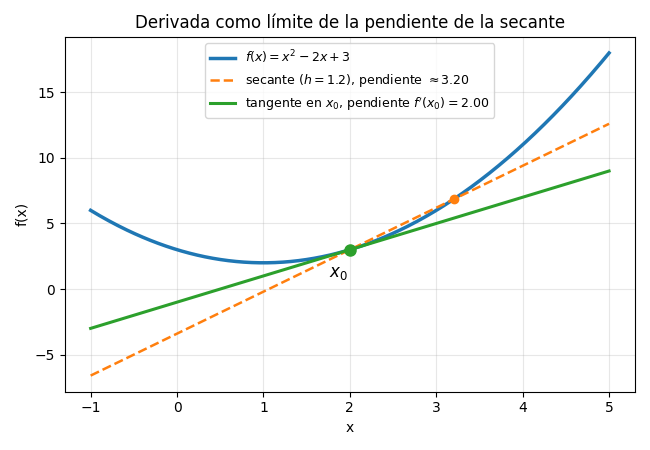
\includegraphics[height=4.5cm,keepaspectratio]{fig01_derivada_tangente.png}
  \end{center}
  \footnotesize Al reducir $h$, la recta secante (naranja) converge a la
  recta tangente (verde) en $x_0$.
\end{frame}

\begin{frame}[fragile]{Derivada en Python: numérica y simbólica}
  \begin{columns}
    \column{0.5\textwidth}
    \textbf{Aproximación numérica} (diferencias finitas):
\begin{lstlisting}
def f(x):
    return x**2 - 2*x + 3

def derivada_numerica(f, x0, h=1e-5):
    return (f(x0 + h) - f(x0)) / h

print(derivada_numerica(f, 2.0))
# -> 2.00001  (exacto: f'(x)=2x-2 -> 2)
\end{lstlisting}
    \column{0.5\textwidth}
    \textbf{Cálculo simbólico} (\texttt{sympy}):
\begin{lstlisting}
import sympy as sp

x = sp.symbols('x')
f = x**2 - 2*x + 3
fprime = sp.diff(f, x)
print(fprime)          # 2*x - 2
print(fprime.subs(x, 2))  # 2
\end{lstlisting}
  \end{columns}
  \vspace{0.2cm}
  \small Script completo: \texttt{scripts/01\_derivada\_tangente.py}
\end{frame}

\begin{frame}{Reglas básicas de derivación (recordatorio)}
  \small
  \begin{columns}
    \column{0.5\textwidth}
    \begin{table}
      \begin{tabular}{ll}
        \toprule
        Función & Derivada \\
        \midrule
        $c$ (constante) & $0$ \\
        $x^n$ & $n\,x^{n-1}$ \\
        $e^x$ & $e^x$ \\
        $\ln x$ & $1/x$ \\
        $\sin x$ & $\cos x$ \\
        $\cos x$ & $-\sin x$ \\
        \bottomrule
      \end{tabular}
    \end{table}
    \column{0.5\textwidth}
    \begin{table}
      \begin{tabular}{ll}
        \toprule
        Regla & Fórmula \\
        \midrule
        Suma & $(f+g)'=f'+g'$ \\
        Producto & $(fg)'=f'g+fg'$ \\
        Cociente & $(f/g)'=\frac{f'g-fg'}{g^2}$ \\
        Cadena & $(f\circ g)'(x)=f'(g(x))g'(x)$ \\
        &\\
        \bottomrule
      \end{tabular}
    \end{table}
  \end{columns}
  \vspace{0.2cm}
  \begin{alertblock}{Para el público no especializado}
    Solo necesitamos saber \emph{qué representa} la derivada (pendiente /
    razón de cambio) y aplicar estas reglas mecánicamente; no se requiere
    dominar todas las técnicas de cálculo.
  \end{alertblock}
\end{frame}

% ==================================================================
\section{Funciones de varias variables y derivadas parciales}
% ==================================================================

\begin{frame}{Funciones de varias variables}
  En optimización casi siempre hay \textbf{más de una variable de
  decisión}: cantidades a producir de varios artículos, dimensiones de una
  pieza, parámetros de un modelo, etc.
  \[
    f: \R^n \to \R, \qquad f(x_1,x_2,\dots,x_n)
  \]
  \begin{exampleblock}{Ejemplo}
    Costo de fabricar una caja rectangular de dimensiones $x,y,z$:
    \[
      f(x,y,z) = 2(xy+yz+xz)\cdot c
    \]
    con $c$ el costo por unidad de área de material.
  \end{exampleblock}
  Nos enfocaremos en $f(x,y): \R^2\to\R$ porque se puede \textbf{visualizar}
  como una superficie; todo generaliza a $n$ variables.
\end{frame}

\begin{frame}{Derivadas parciales: definición}
  \begin{block}{Definición}
    La derivada parcial de $f(x,y)$ respecto a $x$ en $(x_0,y_0)$ es
    \[
      \frac{\partial f}{\partial x}(x_0,y_0) =
      \lim_{h\to 0} \frac{f(x_0+h,y_0)-f(x_0,y_0)}{h}
    \]
    (se deriva respecto a $x$ \textbf{dejando $y$ fija}, y análogamente para
    $\partial f/\partial y$).
  \end{block}
  \begin{itemize}
    \item Notaciones equivalentes: $\dfrac{\partial f}{\partial x} = f_x =
      \partial_x f$.
    \item \textbf{Regla práctica:} se derivan igual que en una variable,
      tratando las demás variables como constantes.
  \end{itemize}
  \begin{exampleblock}{Ejemplo}
    $f(x,y) = x^2 + 2y^2 \ \Rightarrow\ \dfrac{\partial f}{\partial x} = 2x,
    \quad \dfrac{\partial f}{\partial y} = 4y$
  \end{exampleblock}
\end{frame}

\begin{frame}{Interpretación geométrica de la derivada parcial}
  \begin{center}
    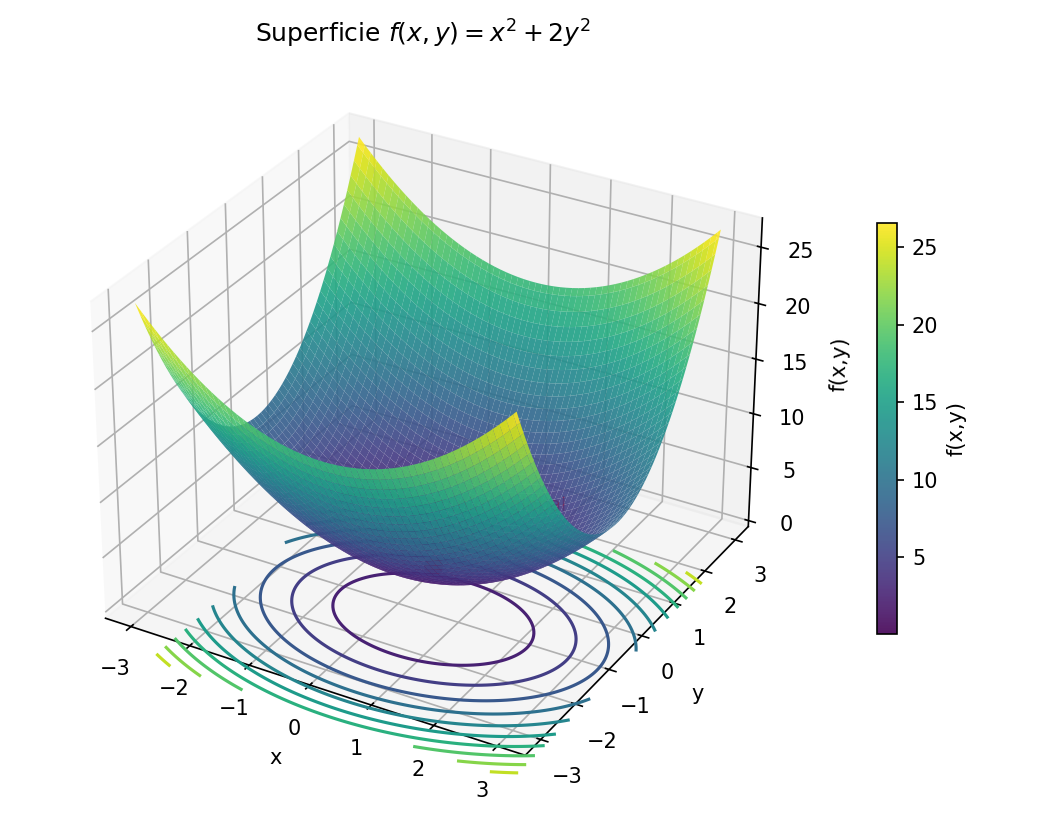
\includegraphics[height=4.5cm,keepaspectratio]{fig02_superficie_3d.png}
  \end{center}
  \footnotesize $\partial f/\partial x$ en $(x_0,y_0)$: pendiente de la curva
  que se obtiene al \textbf{cortar la superficie con el plano $y=y_0$}.
  Análogamente, $\partial f/\partial y$ corresponde al plano $x=x_0$.
\end{frame}

\begin{frame}[fragile]{Generando superficies en Python}
\begin{lstlisting}
import numpy as np
import matplotlib.pyplot as plt

f = lambda x, y: x**2 + 2*y**2

x = np.linspace(-3, 3, 120)
y = np.linspace(-3, 3, 120)
X, Y = np.meshgrid(x, y)      # malla 2D de puntos
Z = f(X, Y)                    # evaluamos f en toda la malla

fig = plt.figure()
ax = fig.add_subplot(111, projection="3d")
ax.plot_surface(X, Y, Z, cmap="viridis")
ax.set_xlabel("x"); ax.set_ylabel("y"); ax.set_zlabel("f(x,y)")
plt.show()
\end{lstlisting}
  \small Script completo: \texttt{scripts/02\_superficie\_3d.py}
\end{frame}

% ==================================================================
\section{El vector gradiente}
% ==================================================================

\begin{frame}{El vector gradiente}
  \begin{block}{Definición}
    El gradiente de $f:\R^n\to\R$ en $\x$ es el vector de todas sus
    derivadas parciales:
    \[
      \grad f(\x) = \left(
        \frac{\partial f}{\partial x_1}, \frac{\partial f}{\partial x_2},
        \dots, \frac{\partial f}{\partial x_n}
      \right)
    \]
  \end{block}
  \begin{itemize}
    \item Para $n=2$: $\grad f(x,y) = \left(\dfrac{\partial f}{\partial x},
      \dfrac{\partial f}{\partial y}\right)$.
    \item El gradiente es un \textbf{campo vectorial}: a cada punto del
      dominio le asocia un vector.
    \item Propiedades: linealidad $\grad(af+bg)=a\grad f + b\grad g$;
      regla del producto $\grad(fg) = g\grad f + f\grad g$.
  \end{itemize}
  \begin{exampleblock}{Ejemplo}
    $f(x,y)=x^2+2y^2 \ \Rightarrow\ \grad f(x,y) = (2x,\,4y)$, y en
    $(1,1)$: $\grad f(1,1) = (2,4)$.
  \end{exampleblock}
\end{frame}

\begin{frame}[fragile]{Gradiente en Python (simbólico y numérico)}
\begin{lstlisting}
import sympy as sp

x, y = sp.symbols('x y')
f = x**2 + 2*y**2
grad_f = [sp.diff(f, v) for v in (x, y)]
print(grad_f)                       # [2*x, 4*y]

punto = {x: 1, y: 1}
grad_en_punto = [g.subs(punto) for g in grad_f]
print(grad_en_punto)                # [2, 4]
\end{lstlisting}
  \vspace{0.2cm}
  \begin{alertblock}{Idea clave}
    El gradiente generaliza la derivada a varias variables: \textbf{apunta
    en la dirección en la que $f$ crece más rápido} (lo demostramos en
    breve) y su magnitud indica \textbf{qué tan rápido} crece en esa
    dirección.
  \end{alertblock}
\end{frame}

% ==================================================================
\section{Curvas de nivel}
% ==================================================================

\begin{frame}{Curvas de nivel (conjuntos de nivel)}
  \begin{block}{Definición}
    La curva (o conjunto) de nivel $c$ de $f:\R^2\to\R$ es
    \[
      \{(x,y)\in\R^2 : f(x,y) = c\}
    \]
    es decir, todos los puntos donde $f$ toma el \textbf{mismo valor}.
  \end{block}
  \begin{itemize}
    \item Son el análogo matemático de las curvas de nivel de un mapa
      topográfico (líneas de igual altitud).
    \item Al variar $c$ se obtiene una familia de curvas que \emph{rebanan} la
      superficie horizontalmente.
    \item Curvas de nivel muy juntas $\Rightarrow$ la función cambia muy
      rápido (pendiente pronunciada); muy separadas $\Rightarrow$ cambia
      lento.
  \end{itemize}
\end{frame}

\begin{frame}{Curvas de nivel y el gradiente}
  \begin{center}
    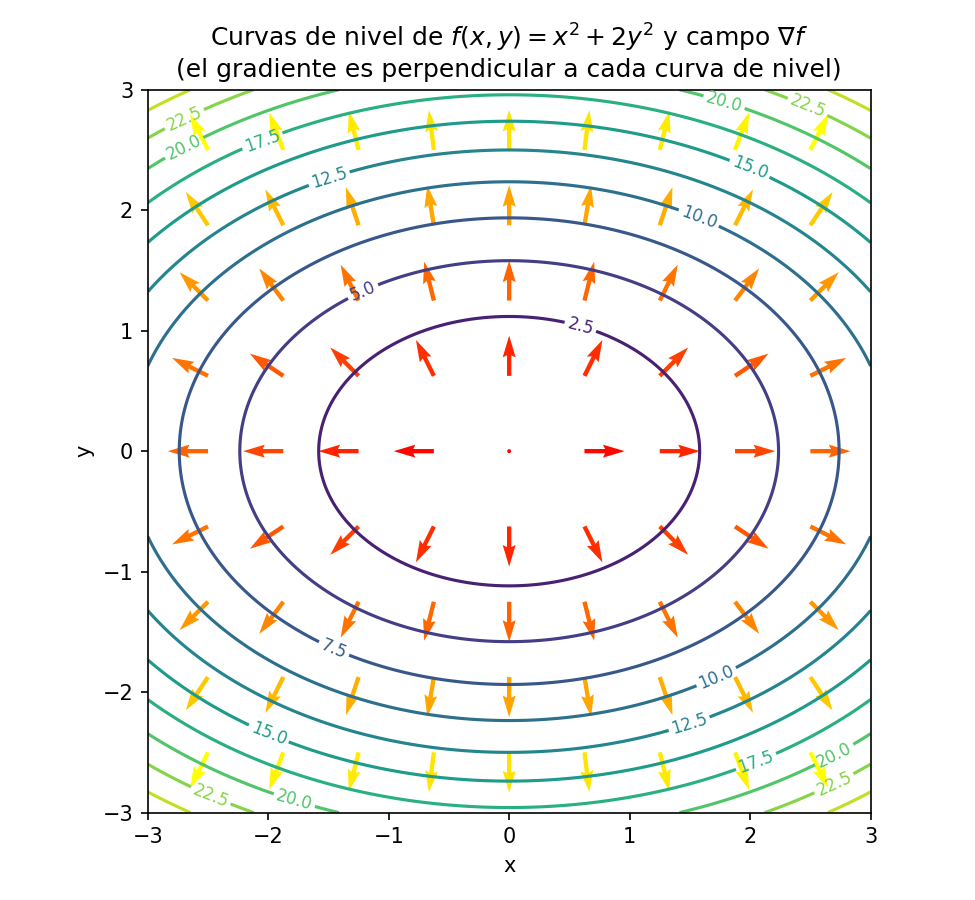
\includegraphics[height=4.2cm,keepaspectratio]{fig03_curvas_nivel_gradiente.png}
  \end{center}
  \begin{alertblock}{Teorema (perpendicularidad)}
    En todo punto, $\grad f$ es \textbf{perpendicular} a la curva de nivel
    que pasa por ese punto, y apunta hacia donde $f$ \textbf{crece}.
  \end{alertblock}
\end{frame}

\begin{frame}[fragile]{Curvas de nivel + gradiente en Python}
\begin{lstlisting}
import numpy as np
import matplotlib.pyplot as plt

f    = lambda x, y: x**2 + 2*y**2
grad = lambda x, y: (2*x, 4*y)

x = np.linspace(-3, 3, 300); y = np.linspace(-3, 3, 300)
X, Y = np.meshgrid(x, y)
plt.contour(X, Y, f(X, Y), levels=12, cmap="viridis")   # curvas de nivel

xg, yg = np.meshgrid(np.linspace(-2.5,2.5,9), np.linspace(-2.5,2.5,9))
U, V = grad(xg, yg)
plt.quiver(xg, yg, U, V)                                  # campo gradiente
plt.gca().set_aspect("equal")
plt.show()
\end{lstlisting}
  \small Script completo: \texttt{scripts/03\_curvas\_nivel\_gradiente.py}
\end{frame}

% ==================================================================
\section{Derivada direccional y máximo crecimiento}
% ==================================================================

\begin{frame}{Derivada direccional: definición}
  \begin{block}{Definición}
    Dado un vector unitario $\u$ ($\|\u\|=1$), la derivada direccional de
    $f$ en $\x_0$ en la dirección $\u$ es
    \[
      D_\u f(\x_0) = \lim_{t\to 0} \frac{f(\x_0+t\u)-f(\x_0)}{t}
    \]
  \end{block}
  \begin{itemize}
    \item Mide qué tan rápido cambia $f$ si nos movemos desde $\x_0$ en la
      dirección $\u$.
    \item Caso particular: si $\u=(1,0)$, $D_\u f = \partial f/\partial x$.
  \end{itemize}
  \begin{alertblock}{Fórmula práctica (si $f$ es diferenciable)}
    \[
      D_\u f(\x_0) = \grad f(\x_0) \cdot \u
    \]
    ¡No hace falta calcular un límite nuevo cada vez! Basta con el
    gradiente.
  \end{alertblock}
\end{frame}

\begin{frame}{Derivada direccional: visualización}
  \begin{center}
    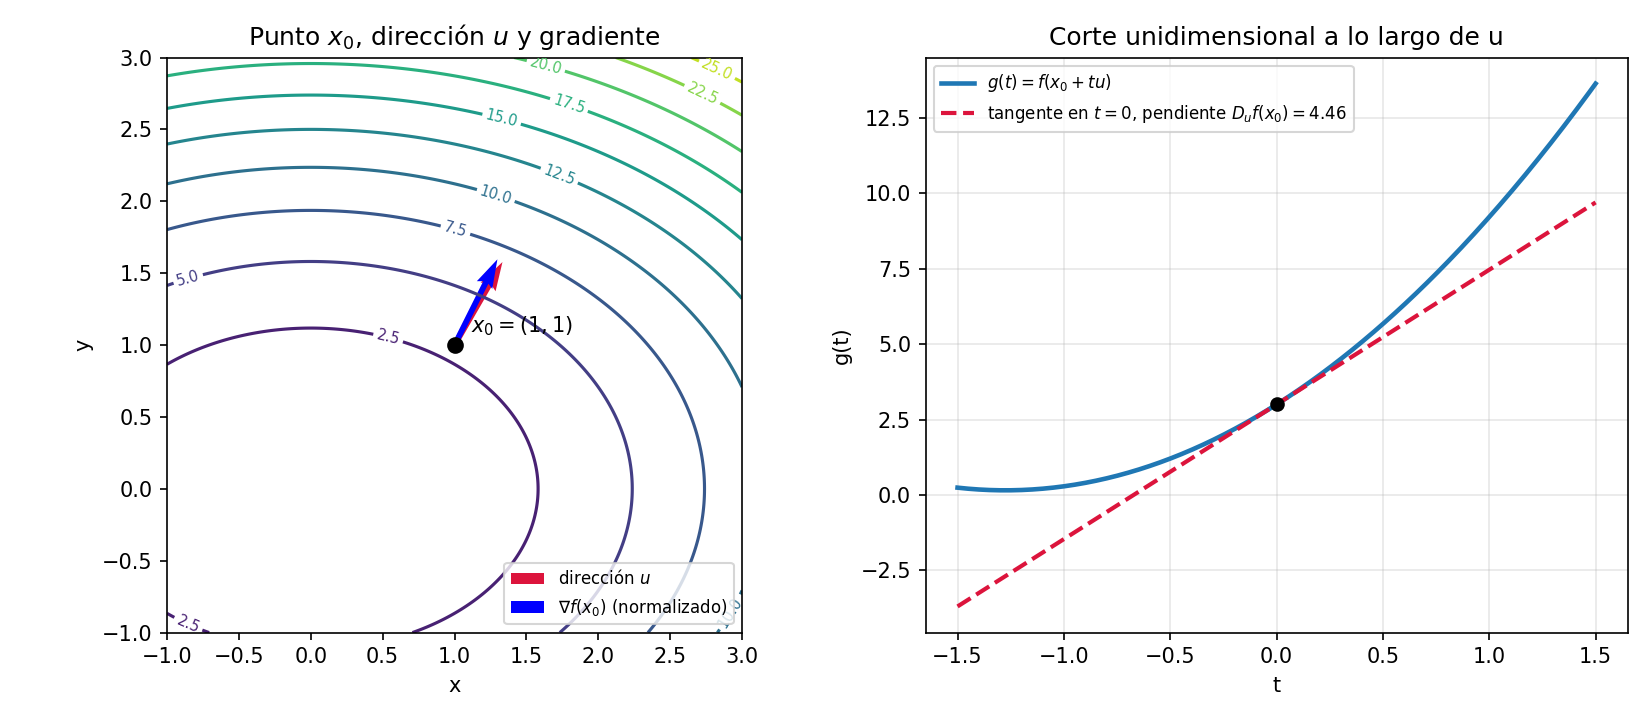
\includegraphics[height=4.6cm,keepaspectratio]{fig05_derivada_direccional.png}
  \end{center}
  \footnotesize Izquierda: punto $x_0$, dirección $u$ y $\grad f(x_0)$
  sobre las curvas de nivel. Derecha: corte $g(t)=f(x_0+tu)$; la pendiente
  de su tangente en $t=0$ es $D_uf(x_0)$.
\end{frame}

\begin{frame}{El gradiente como dirección de máximo crecimiento}
  Usando $D_\u f(\x_0) = \grad f(\x_0)\cdot \u = \|\grad f(\x_0)\|\,\|\u\|
  \cos\theta$, con $\theta$ el ángulo entre $\grad f(\x_0)$ y $\u$, y como
  $\|\u\|=1$:
  \[
    D_\u f(\x_0) = \|\grad f(\x_0)\| \cos\theta
  \]
  \begin{alertblock}{Consecuencia}
    $D_\u f(\x_0)$ es \textbf{máxima} cuando $\cos\theta=1$, es decir,
    cuando $\u$ apunta \textbf{en la misma dirección que $\grad f(\x_0)$}.
    \begin{itemize}
      \item Dirección de \textbf{máximo ascenso}: $\u = \grad f(\x_0)/\|\grad f(\x_0)\|$.
      \item Dirección de \textbf{máximo descenso}: $\u = -\grad f(\x_0)/\|\grad f(\x_0)\|$.
    \end{itemize}
  \end{alertblock}
  \small Este hecho es la base del \textbf{método de descenso de gradiente},
  que veremos en una próxima clase: para minimizar, uno se mueve
  repetidamente en la dirección $-\grad f(\x)$.
\end{frame}

\begin{frame}{Gradientes superpuestos sobre la superficie}
  \begin{center}
    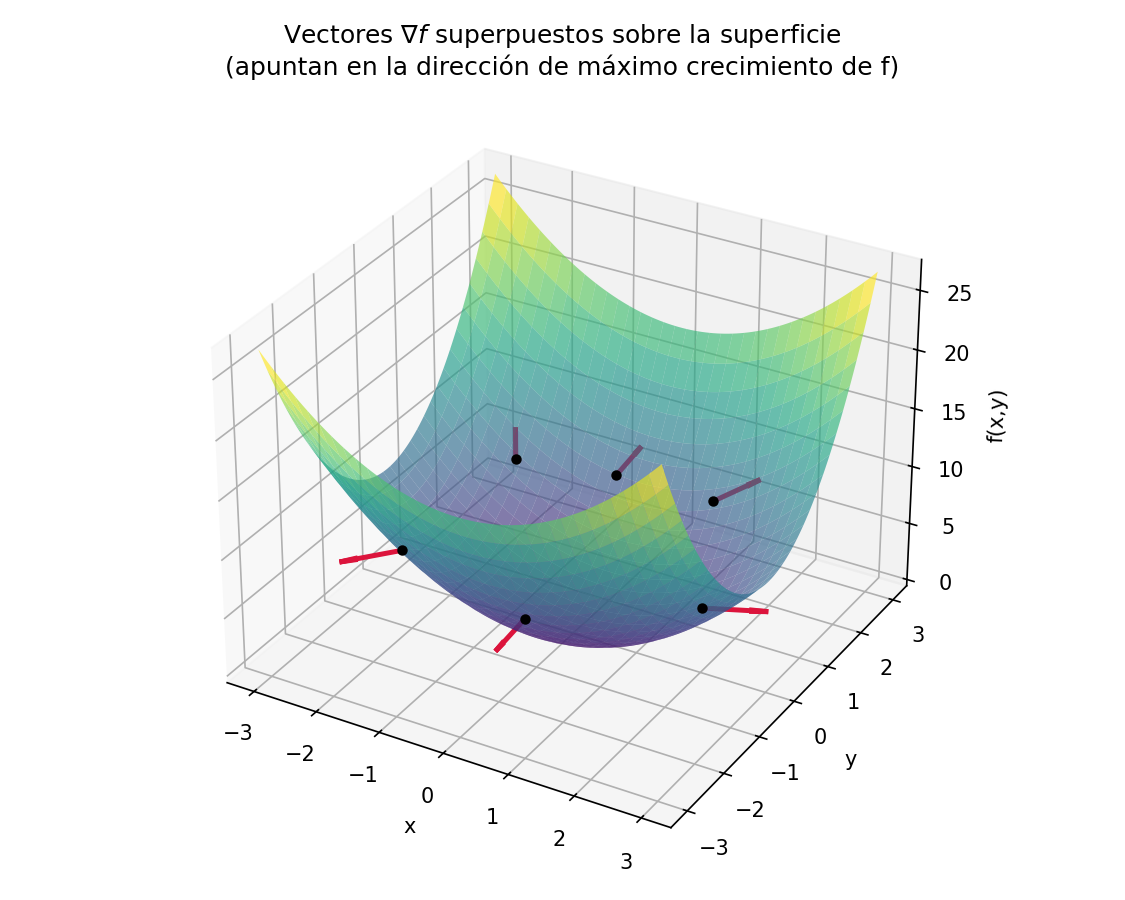
\includegraphics[height=4.3cm,keepaspectratio]{fig04_gradiente_superficie_3d.png}
  \end{center}
  \footnotesize En cada punto de la superficie, el vector gradiente
  (proyectado en el plano $xy$) apunta hacia donde $f$ aumenta más
  rápido: aquí, siempre \emph{cuesta arriba} alejándose del mínimo en el
  origen.
\end{frame}

% ==================================================================
\section{Monotonía}
% ==================================================================

\begin{frame}{Monotonía}
  \begin{block}{Una variable}
    $f$ es \textbf{creciente} en un intervalo si $f'(x) > 0$ allí, y
    \textbf{decreciente} si $f'(x) < 0$. Si $f'(x)=0$ en un intervalo, $f$
    es constante allí.
  \end{block}
  \begin{block}{Varias variables (a lo largo de una dirección)}
    $f$ es creciente en $\x_0$ en la dirección $\u$ si $D_\u f(\x_0) > 0$,
    y decreciente si $D_\u f(\x_0) < 0$.
  \end{block}
  \begin{exampleblock}{Ejemplo}
    Para $f(x,y)=x^2+2y^2$ en $\x_0=(1,1)$, moverse en la dirección
    $\u=\grad f(\x_0)/\|\grad f(\x_0)\|$ hace crecer $f$ lo más rápido
    posible ($D_\u f(\x_0) = \|\grad f(\x_0)\| > 0$); moverse en $-\u$ la
    hace decrecer lo más rápido posible.
  \end{exampleblock}
\end{frame}

% ==================================================================
\section{Puntos críticos}
% ==================================================================

\begin{frame}{Puntos críticos: condición necesaria}
  \small
  \begin{block}{Definición}
    $\x^*$ es un \textbf{punto crítico} (o estacionario) de $f$ si
    \[
      \grad f(\x^*) = \mathbf{0}
    \]
    (en una variable: $f'(x^*)=0$).
  \end{block}
  \begin{alertblock}{Teorema (condición necesaria de primer orden)}
    Si $\x^*$ es un mínimo o máximo \textbf{local} de $f$ (diferenciable, sin
    restricciones), entonces $\x^*$ es un punto crítico.
  \end{alertblock}
  \begin{itemize}
    \item \textbf{No todo punto crítico es un mínimo o máximo}: también
      puede ser un \textbf{punto de silla} (más adelante).
    \item Buscar óptimos $\Rightarrow$ primero encontrar dónde $\grad
      f(\x)=\mathbf{0}$, y luego clasificar cada punto crítico.
  \end{itemize}
  \begin{exampleblock}{Ejemplo}
    $f(x,y)=x^2+2y^2$: $\grad f = (2x,4y) = (0,0) \Rightarrow (x,y)=(0,0)$
    es el único punto crítico.
  \end{exampleblock}
\end{frame}

% ==================================================================
\section{La matriz Hessiana}
% ==================================================================

\begin{frame}{La matriz Hessiana}
  \begin{block}{Definición}
    La Hessiana de $f:\R^n\to\R$ (dos veces diferenciable) es la matriz de
    segundas derivadas parciales:
    \[
      \Hess(\x) = \begin{pmatrix}
        \dfrac{\partial^2 f}{\partial x_1^2} & \cdots & \dfrac{\partial^2 f}{\partial x_1 \partial x_n} \\
        \vdots & \ddots & \vdots \\
        \dfrac{\partial^2 f}{\partial x_n \partial x_1} & \cdots & \dfrac{\partial^2 f}{\partial x_n^2}
      \end{pmatrix}
    \]
    Bajo condiciones usuales de continuidad, $\Hess$ es \textbf{simétrica}.
  \end{block}
  \begin{exampleblock}{Ejemplo}
    $f(x,y)=x^2+2y^2 \ \Rightarrow\ \Hess = \begin{pmatrix} 2 & 0 \\ 0 & 4 \end{pmatrix}$
    (constante en todo el dominio, por ser $f$ cuadrática).
  \end{exampleblock}
\end{frame}

\begin{frame}{Matrices definidas positivas / negativas}
  \begin{block}{Definición}
    Una matriz simétrica $H$ es:
    \begin{itemize}
      \item \textbf{Definida positiva} si $\dd^\top H \dd > 0$ para todo
        $\dd\neq\mathbf{0}$ $\Leftrightarrow$ todos sus autovalores $>0$.
      \item \textbf{Definida negativa} si $\dd^\top H \dd < 0$ para todo
        $\dd\neq\mathbf{0}$ $\Leftrightarrow$ todos sus autovalores $<0$.
      \item \textbf{Indefinida} si toma ambos signos $\Leftrightarrow$
        tiene autovalores de ambos signos.
    \end{itemize}
  \end{block}
  \begin{alertblock}{Criterio práctico en $2\times 2$}
    Para $H=\begin{pmatrix}a&b\\b&c\end{pmatrix}$, con
    $\det H = ac-b^2$:
    \begin{itemize}
      \item $\det H>0$ y $a>0$ $\Rightarrow$ definida positiva.
      \item $\det H>0$ y $a<0$ $\Rightarrow$ definida negativa.
      \item $\det H<0$ $\Rightarrow$ indefinida (punto de silla).
    \end{itemize}
  \end{alertblock}
\end{frame}

\begin{frame}{Clasificación de puntos críticos}
  \begin{block}{Criterio de la segunda derivada}
    Sea $\x^*$ un punto crítico ($\grad f(\x^*)=\mathbf 0$):
    \begin{itemize}
      \item $\Hess(\x^*)$ definida positiva $\Rightarrow$ \textbf{mínimo
        local} estricto.
      \item $\Hess(\x^*)$ definida negativa $\Rightarrow$ \textbf{máximo
        local} estricto.
      \item $\Hess(\x^*)$ indefinida $\Rightarrow$ \textbf{punto de silla}
        (ni máximo ni mínimo).
      \item $\Hess(\x^*)$ semidefinida (con autovalor 0) $\Rightarrow$ el
        criterio \textbf{no decide}; se requiere más análisis.
    \end{itemize}
  \end{block}
  \small (En una variable, esto es el conocido criterio $f''(x^*)>0
  \Rightarrow$ mínimo, $f''(x^*)<0\Rightarrow$ máximo.)
\end{frame}

\begin{frame}{Los tres casos, visualizados}
  \begin{center}
    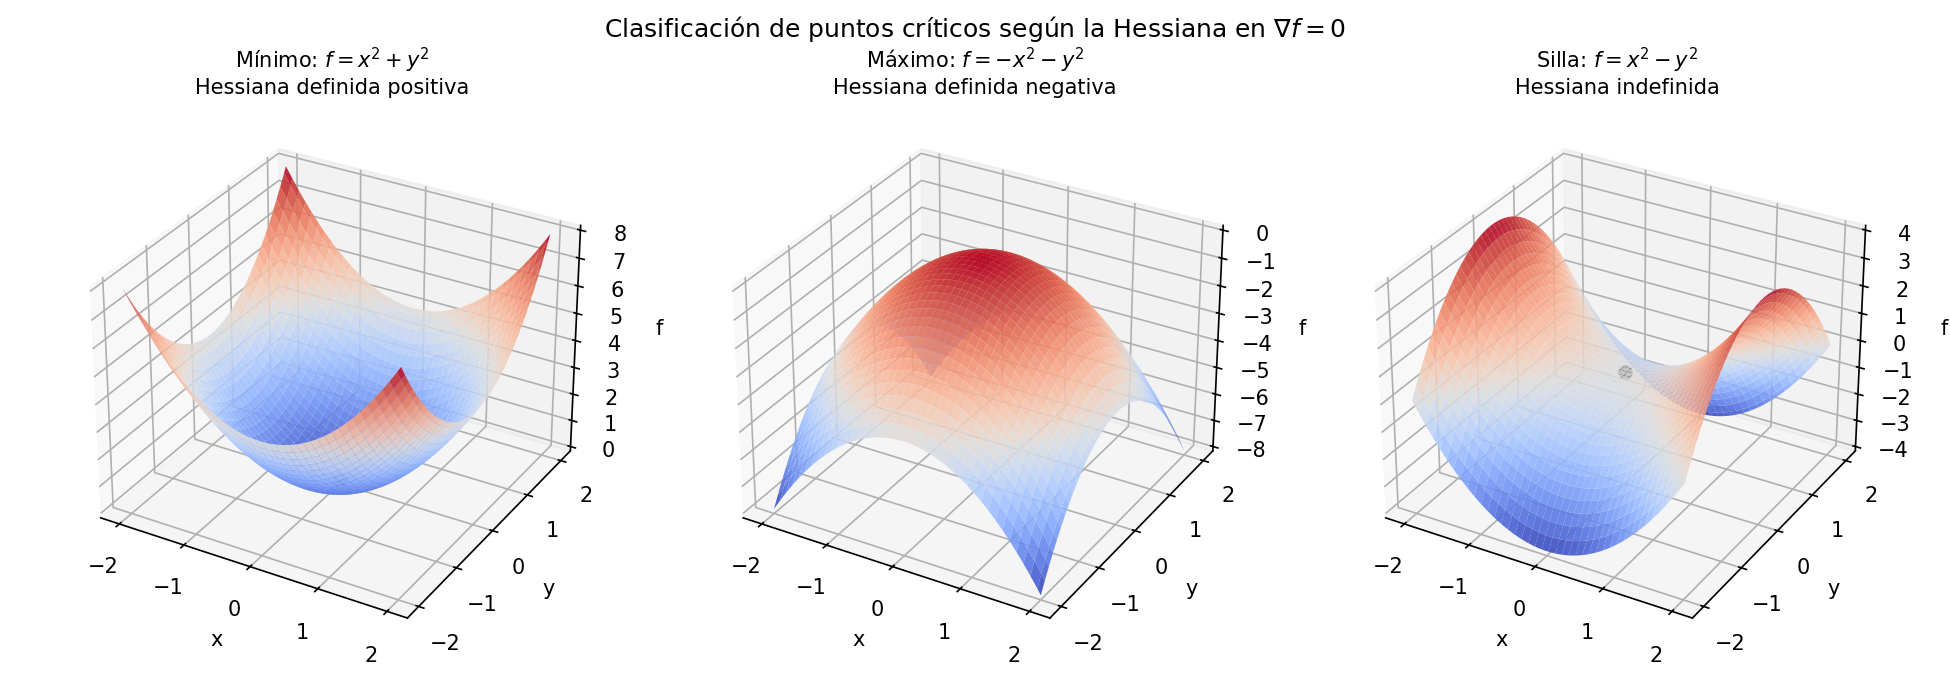
\includegraphics[width=0.98\textwidth]{fig06_puntos_criticos.png}
  \end{center}
\end{frame}

\begin{frame}[fragile]{Clasificar puntos críticos en Python}
\begin{lstlisting}
import numpy as np

H = np.array([[2, 0],
              [0, -4]])                 # Hessiana en el punto critico

eigvals = np.linalg.eigvalsh(H)         # autovalores (H simetrica)
print(eigvals)                          # [-4.  2.]

if np.all(eigvals > 0):
    print("minimo local")
elif np.all(eigvals < 0):
    print("maximo local")
elif np.any(eigvals > 0) and np.any(eigvals < 0):
    print("punto de silla")
else:
    print("caso no decidido por el criterio (autovalor 0)")
\end{lstlisting}
\end{frame}

% ==================================================================
\section{Serie de Taylor}
% ==================================================================

\begin{frame}{Serie de Taylor en una variable}
  \begin{block}{Idea}
    Aproximar $f$ cerca de $x_0$ mediante un polinomio construido con sus
    derivadas en $x_0$:
    \[
      f(x) \approx f(x_0) + f'(x_0)(x-x_0) + \frac{f''(x_0)}{2!}(x-x_0)^2 +
      \dots
    \]
  \end{block}
  \begin{itemize}
    \item \textbf{Orden 1} (lineal): $f(x)\approx f(x_0)+f'(x_0)(x-x_0)$
      — es la recta tangente.
    \item \textbf{Orden 2} (cuadrático):
      $f(x)\approx f(x_0)+f'(x_0)(x-x_0)+\tfrac12 f''(x_0)(x-x_0)^2$ —
      captura también la \textbf{curvatura}.
    \item Cuanto mayor el orden, mejor la aproximación \textbf{cerca} de
      $x_0$ (pero puede empeorar lejos de $x_0$).
  \end{itemize}
\end{frame}

\begin{frame}{Serie de Taylor: visualización}
  \begin{center}
    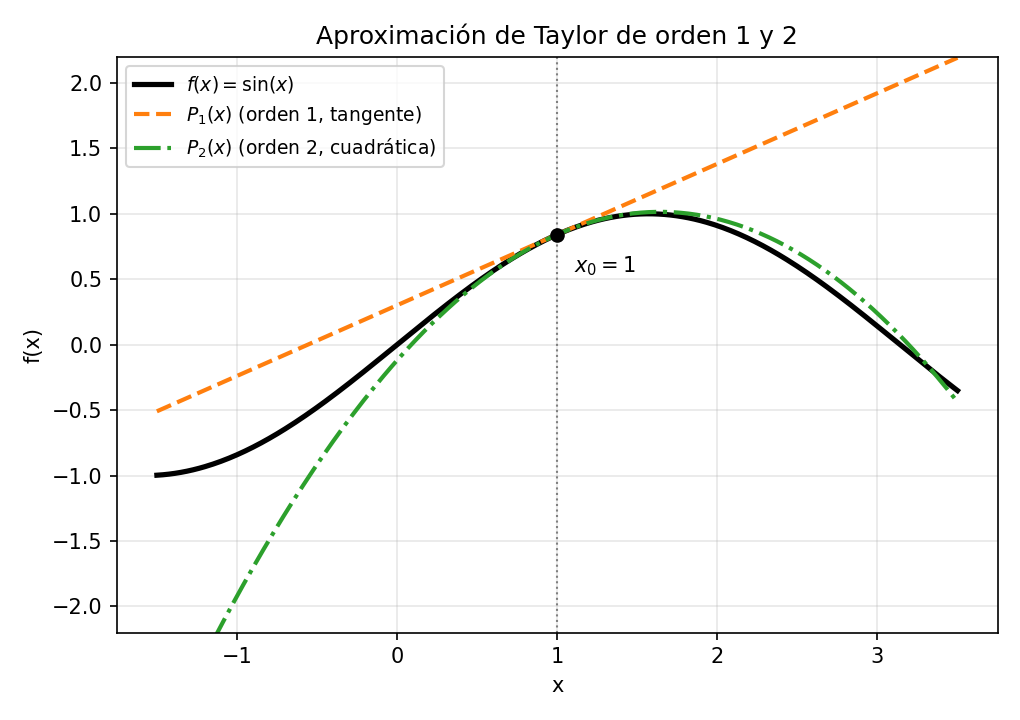
\includegraphics[width=0.62\textwidth]{fig07_taylor.png}
  \end{center}
  \footnotesize $f(x)=\sin(x)$ cerca de $x_0=1$: la aproximación cuadrática
  $P_2$ sigue a $f$ mucho más de cerca que la lineal $P_1$.
\end{frame}

\begin{frame}{Serie de Taylor multivariable}
  Para $f:\R^n\to\R$, alrededor de $\x_0$ y con incremento $\dd$:
  \[
    f(\x_0+\dd) \approx \underbrace{f(\x_0)}_{\text{orden 0}} +
    \underbrace{\grad f(\x_0)^\top \dd}_{\text{orden 1}} +
    \underbrace{\tfrac12\, \dd^\top \Hess(\x_0)\, \dd}_{\text{orden 2}}
  \]
  \begin{alertblock}{Por qué importa en optimización}
    La aproximación de \textbf{orden 2} es un \textbf{modelo cuadrático
    local} de $f$: los métodos de optimización tipo \textbf{Newton}
    minimizan ese modelo cuadrático en cada paso en lugar de $f$
    directamente (lo veremos en una próxima clase).
  \end{alertblock}
  \begin{itemize}
    \item Si $\x_0$ es un punto crítico ($\grad f(\x_0)=\mathbf 0$), el
      modelo se reduce a $f(\x_0) + \tfrac12 \dd^\top \Hess(\x_0)\dd$ — por
      eso la Hessiana clasifica el punto crítico.
  \end{itemize}
\end{frame}

\begin{frame}[fragile]{Taylor en Python}
\begin{lstlisting}
import numpy as np

f       = np.sin
fprime  = np.cos
fsecond = lambda x: -np.sin(x)

x0 = 1.0
x  = np.linspace(x0 - 2, x0 + 2, 200)

P1 = f(x0) + fprime(x0) * (x - x0)                            # orden 1
P2 = P1 + 0.5 * fsecond(x0) * (x - x0)**2                     # orden 2
\end{lstlisting}
  \small Script completo: \texttt{scripts/07\_taylor\_series.py}
\end{frame}

% ==================================================================
\section{Convexidad}
% ==================================================================

\begin{frame}{Conjuntos y funciones convexas}
  \begin{block}{Conjunto convexo}
    $\Omega\subseteq\R^n$ es convexo si el segmento que une dos puntos
    cualesquiera de $\Omega$ está contenido en $\Omega$:
    \[
      \x_1,\x_2\in\Omega,\ t\in[0,1] \ \Rightarrow\ t\x_1+(1-t)\x_2\in\Omega
    \]
  \end{block}
  \begin{block}{Función convexa}
    $f:\Omega\to\R$ (con $\Omega$ convexo) es convexa si
    \[
      f(t\x_1+(1-t)\x_2) \ \le\ t f(\x_1) + (1-t) f(\x_2)
      \qquad \forall\, \x_1,\x_2\in\Omega,\ t\in[0,1]
    \]
  \end{block}
  \footnotesize Interpretación: la \textbf{cuerda} entre dos puntos de la
  gráfica queda \textbf{siempre por encima} (o sobre) la función. Si la
  desigualdad es estricta para $\x_1\neq\x_2$, $t\in(0,1)$, es
  \textbf{estrictamente convexa}.
\end{frame}

\begin{frame}{Convexidad: visualización}
  \begin{center}
    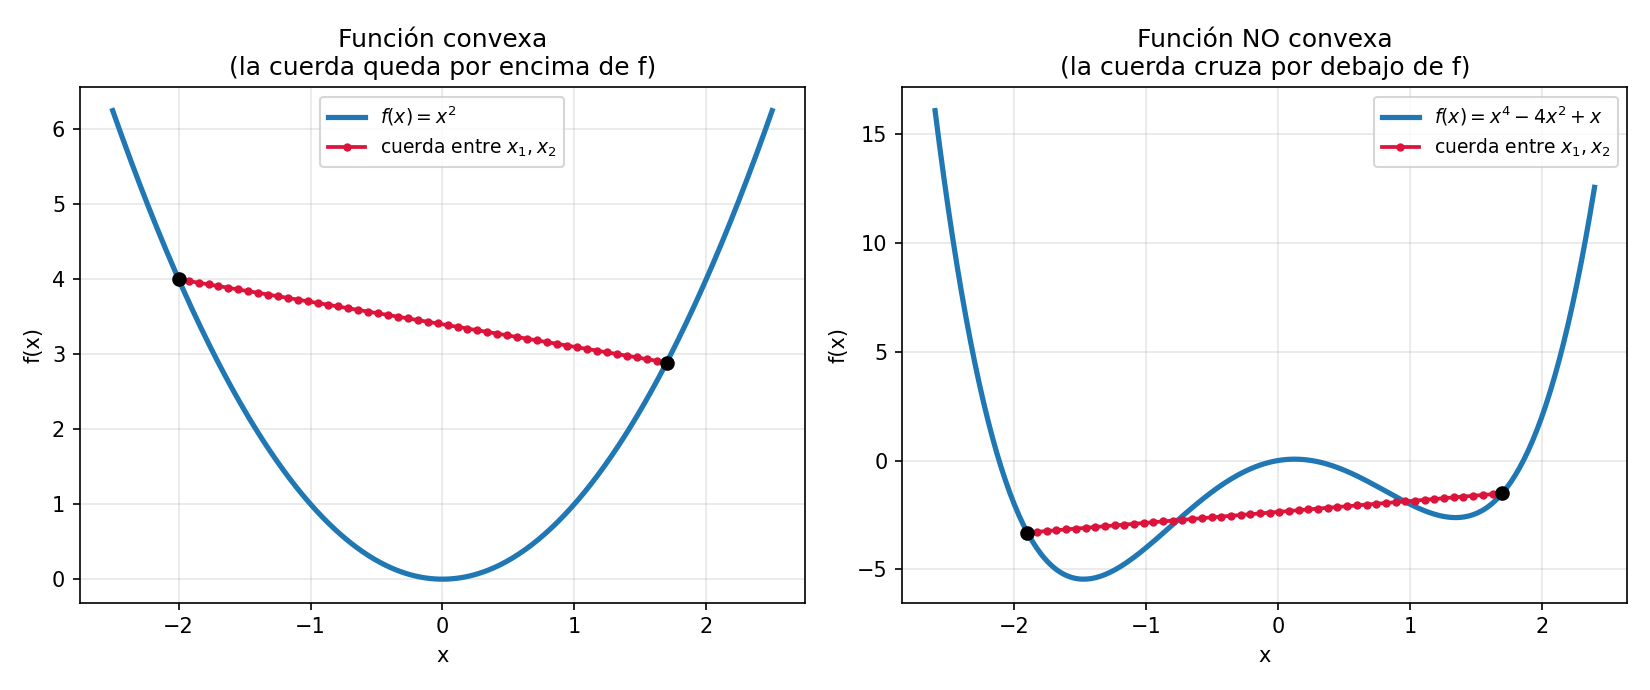
\includegraphics[width=0.95\textwidth]{fig08_convexidad.png}
  \end{center}
\end{frame}

\begin{frame}{Caracterizaciones de convexidad}
  Si $f$ es diferenciable, son equivalentes a la definición anterior:
  \begin{block}{Caracterización de primer orden}
    \[
      f(\mathbf{y}) \ge f(\x) + \grad f(\x)^\top(\mathbf{y}-\x)
      \qquad \forall\, \x,\mathbf y \in \Omega
    \]
    (la función siempre queda \textbf{por encima} de su plano tangente).
  \end{block}
  \begin{block}{Caracterización de segundo orden}
    Si $f$ es dos veces diferenciable, $f$ es convexa
    $\Leftrightarrow$ $\Hess(\x)$ es \textbf{semidefinida positiva} para
    todo $\x\in\Omega$ (y \emph{definida} positiva $\Rightarrow$
    estrictamente convexa).
  \end{block}
  \small En una variable: $f$ convexa $\Leftrightarrow$ $f''(x)\ge 0$ en
  todo el dominio.
\end{frame}

\begin{frame}{¿Por qué importa la convexidad?}
  \begin{alertblock}{Teorema central de la optimización convexa}
    Si $f$ es convexa (sobre $\Omega$ convexo), entonces \textbf{todo mínimo
    local es también un mínimo global}.
  \end{alertblock}
  \begin{itemize}
    \item Elimina el problema de quedar \emph{atrapado} en un mínimo local
      subóptimo.
    \item Es la razón por la que la \textbf{optimización convexa} es una
      de las áreas mejor entendidas y más usadas (regresión, SVM, control,
      finanzas, muchos problemas de ingeniería).
    \item Muchos algoritmos (descenso de gradiente, Newton) tienen
      \textbf{garantías teóricas fuertes} solo cuando $f$ es convexa.
  \end{itemize}
  \begin{exampleblock}{Ejemplo}
    $f(x,y)=x^2+2y^2$ tiene $\Hess=\begin{pmatrix}2&0\\0&4\end{pmatrix}$,
    definida positiva en todo punto $\Rightarrow$ $f$ es (estrictamente)
    convexa $\Rightarrow$ su único punto crítico $(0,0)$ es el mínimo
    global.
  \end{exampleblock}
\end{frame}

\begin{frame}[fragile]{Verificar convexidad en Python (numéricamente)}
\begin{lstlisting}
import numpy as np

def es_semidef_positiva(H, tol=1e-9):
    autovalores = np.linalg.eigvalsh(H)
    return np.all(autovalores >= -tol)

H = np.array([[2, 0],
              [0, 4]])
print(es_semidef_positiva(H))     # True  -> f convexa en ese punto
\end{lstlisting}
  \small Script completo: \texttt{scripts/08\_convexidad.py}
\end{frame}

% ==================================================================
\section{Máximos y mínimos: locales vs. globales}
% ==================================================================

\begin{frame}{Mínimos y máximos: local vs. global}
  \begin{block}{Definiciones}
    $\x^*\in\Omega$ es:
    \begin{itemize}
      \item \textbf{mínimo local} si $f(\x^*)\le f(\x)$ para todo $\x$ en
        un entorno de $\x^*$;
      \item \textbf{mínimo global} si $f(\x^*)\le f(\x)$ para \textbf{todo}
        $\x\in\Omega$.
    \end{itemize}
    (análogo para máximos, invirtiendo la desigualdad).
  \end{block}
  \begin{alertblock}{Teorema de Weierstrass (existencia)}
    Si $\Omega$ es \textbf{compacto} (cerrado y acotado) y $f$ es
    \textbf{continua}, entonces $f$ alcanza un mínimo global y un máximo
    global en $\Omega$.
  \end{alertblock}
  \small Sin compacidad no hay garantía: por ejemplo $f(x)=x$ en $\R$ no
  tiene mínimo ni máximo.
\end{frame}

\begin{frame}{Ejemplo: varios mínimos locales}
  \begin{center}
    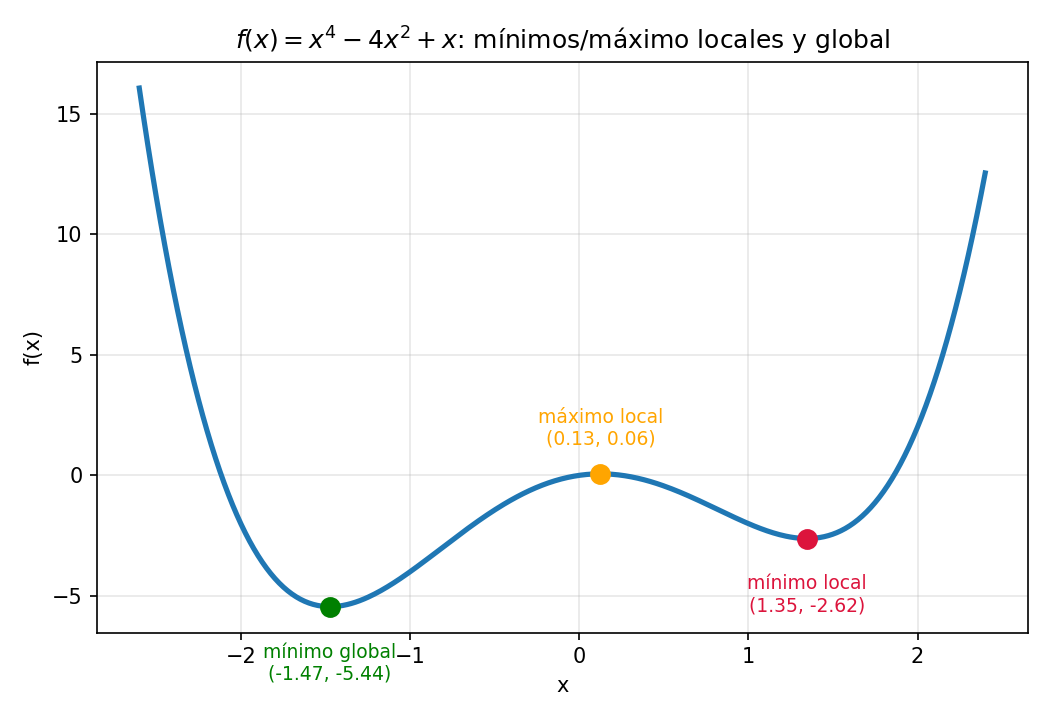
\includegraphics[width=0.62\textwidth]{fig09_min_local_global.png}
  \end{center}
  \footnotesize $f(x)=x^4-4x^2+x$ tiene dos mínimos locales, pero solo uno
  es el mínimo \textbf{global} (el de menor valor de $f$); en medio hay un
  máximo local. Esta función \textbf{no es convexa} (por eso puede tener
  más de un mínimo local).
\end{frame}

\begin{frame}[fragile]{Ubicar puntos críticos en Python}
\begin{lstlisting}
import numpy as np

# f(x) = x^4 - 4x^2 + x  ->  f'(x) = 4x^3 - 8x + 1
coef_fprime = [4, 0, -8, 1]
raices = np.roots(coef_fprime)
raices = np.sort(raices[np.isreal(raices)].real)

fsecond = lambda x: 12*x**2 - 8
for r in raices:
    tipo = "minimo" if fsecond(r) > 0 else "maximo"
    print(f"x*={r:.3f}  tipo={tipo}  f(x*)={r**4-4*r**2+r:.3f}")
\end{lstlisting}
  \small Script completo: \texttt{scripts/09\_min\_local\_global.py}
\end{frame}

% ==================================================================
\section{Optimización sin restricciones: síntesis}
% ==================================================================

\begin{frame}{Condiciones de optimalidad sin restricciones}
  \begin{block}{Para $\min_{\x\in\R^n} f(\x)$, con $f$ dos veces diferenciable}
    \begin{itemize}
      \item \textbf{Condición necesaria de primer orden:} si $\x^*$ es
        mínimo local, $\grad f(\x^*)=\mathbf 0$.
      \item \textbf{Condición suficiente de segundo orden:} si
        $\grad f(\x^*)=\mathbf 0$ y $\Hess(\x^*)$ es definida positiva,
        entonces $\x^*$ es mínimo local estricto.
      \item Si además $f$ es \textbf{convexa}, todo mínimo local
        (equivalentemente, todo punto con $\grad f=\mathbf 0$) es
        \textbf{mínimo global}.
    \end{itemize}
  \end{block}
  \begin{alertblock}{Receta general (a mano)}
    1) Calcular $\grad f$ y resolver $\grad f(\x)=\mathbf 0$ (puntos
    críticos). \quad 2) Calcular $\Hess$ en cada punto crítico y
    clasificarlo. \quad 3) Si aplica, verificar convexidad para garantizar
    optimalidad global.
  \end{alertblock}
\end{frame}

% ==================================================================
\section{Restricciones de igualdad: multiplicadores de Lagrange}
% ==================================================================

\begin{frame}{Optimización con restricciones de igualdad}
  \[
    \min_{\x\in\R^n} f(\x) \quad \text{s.a.} \quad h(\x) = 0
  \]
  \begin{itemize}
    \item $h:\R^n\to\R$ define una \textbf{superficie/curva de
      restricción}: solo podemos buscar el óptimo \textbf{sobre} ella.
    \item Ejemplo: maximizar el área de un rectángulo de lados $x,y$ con
      perímetro fijo $2x+2y=P$.
  \end{itemize}
  \begin{alertblock}{Idea geométrica}
    En el óptimo restringido $\x^*$, \textbf{no puede mejorar} moverse a lo
    largo de la restricción; esto ocurre exactamente cuando $\grad
    f(\x^*)$ es \textbf{paralelo} a $\grad h(\x^*)$ (perpendicular ambos a
    la curva de restricción en $\x^*$).
  \end{alertblock}
\end{frame}

\begin{frame}{El método de los multiplicadores de Lagrange}
  \begin{block}{Función Lagrangiana}
    \[
      \mathcal L(\x,\lambda) = f(\x) - \lambda\, h(\x)
    \]
  \end{block}
  \begin{block}{Condiciones necesarias de primer orden}
    \[
      \grad_\x \mathcal L = \mathbf 0 \ \Longrightarrow\ \grad f(\x^*) =
      \lambda \grad h(\x^*), \qquad h(\x^*) = 0
    \]
  \end{block}
  \begin{itemize}
    \item $\lambda$ (\textbf{multiplicador de Lagrange}) mide cuánto
      cambiaría el óptimo de $f$ si se relajara ligeramente la restricción.
    \item Da un sistema de $n+1$ ecuaciones ($\grad f=\lambda\grad h$ y
      $h=0$) con $n+1$ incógnitas ($\x^*,\lambda$).
  \end{itemize}
\end{frame}

\begin{frame}{Ejemplo resuelto}
  \[
    \min_{x,y} \ f(x,y)=x^2+y^2 \qquad \text{s.a.} \qquad h(x,y)=x+y-4=0
  \]
  \[
    \grad f = (2x,2y), \quad \grad h = (1,1)
    \ \Rightarrow\ 2x=\lambda,\ 2y=\lambda \ \Rightarrow\ x=y
  \]
  Con $x+y=4$: $x=y=2$, $\lambda=4$.
  \begin{center}
    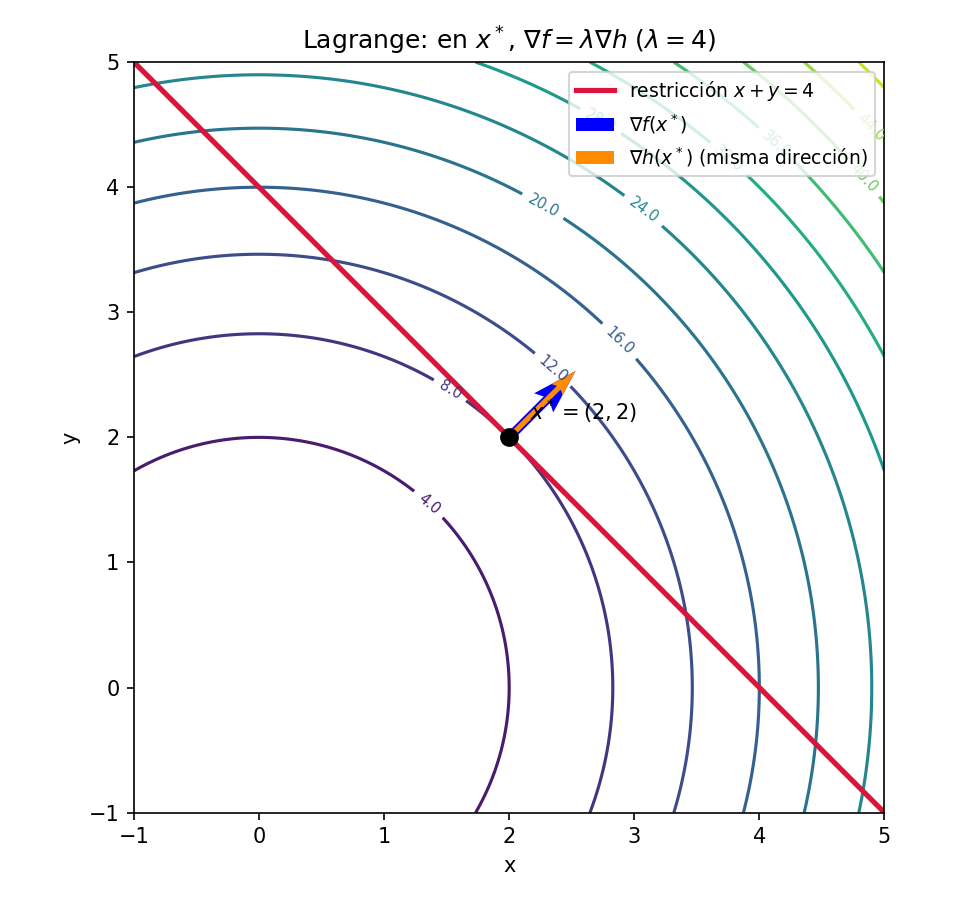
\includegraphics[height=3.6cm,keepaspectratio]{fig10_lagrange_igualdad.png}
  \end{center}
\end{frame}

\begin{frame}[fragile]{Lagrange en Python (con \texttt{sympy})}
\begin{lstlisting}
import sympy as sp

x, y, lam = sp.symbols('x y lambda')
f = x**2 + y**2
h = x + y - 4

L = f - lam*h
ecuaciones = [sp.diff(L, v) for v in (x, y, lam)]
solucion = sp.solve(ecuaciones, (x, y, lam))
print(solucion)     # {x: 2, y: 2, lambda: 4}
\end{lstlisting}
  \small Script completo (versión gráfica):
  \texttt{scripts/10\_lagrange\_igualdad.py}
\end{frame}

% ==================================================================
\section{Restricciones de desigualdad: introducción a KKT}
% ==================================================================

\begin{frame}{Optimización con restricciones de desigualdad}
  \[
    \min_{\x\in\R^n} f(\x) \quad \text{s.a.} \quad g(\x) \le 0
  \]
  \begin{itemize}
    \item El conjunto factible es una \textbf{región} (no solo una curva),
      p.\,ej.\ $g(\x)\le 0$ recorta un semiespacio, un semiplano curvo, etc.
    \item En el óptimo, la restricción puede estar:
      \begin{itemize}
        \item \textbf{activa}: $g(\x^*)=0$ (el óptimo está sobre la
          frontera);
        \item \textbf{inactiva}: $g(\x^*)<0$ (el óptimo está en el
          interior — la restricción \emph{no estorba}, como si no existiera).
      \end{itemize}
  \end{itemize}
  \begin{alertblock}{Idea clave}
    Si el mínimo \emph{sin} restricciones ya es factible, la restricción de
    desigualdad es inactiva y el problema se resuelve como sin
    restricciones. Si no, el óptimo se \emph{empuja} hasta la frontera.
  \end{alertblock}
\end{frame}

\begin{frame}{Condiciones de Karush--Kuhn--Tucker (KKT)}
  Para $\min f(\x)$ s.a. $g(\x)\le 0$ (caso con una sola restricción, por
  simplicidad), $\x^*$ óptimo requiere que exista $\mu^*\ge 0$ con:
  \begin{block}{Condiciones KKT}
    \begin{enumerate}
      \item \textbf{Estacionariedad:} $\grad f(\x^*) + \mu^* \grad g(\x^*) = \mathbf 0$
      \item \textbf{Factibilidad primal:} $g(\x^*) \le 0$
      \item \textbf{Factibilidad dual:} $\mu^* \ge 0$
      \item \textbf{Holgura complementaria:} $\mu^*\, g(\x^*) = 0$
    \end{enumerate}
  \end{block}
  \footnotesize La condición 4 formaliza la idea de activa/inactiva: si
  $g(\x^*)<0$ (inactiva) entonces $\mu^*=0$ forzosamente (no \emph{empuja}); si
  $\mu^*>0$ entonces $g(\x^*)=0$ (activa). Estas condiciones son la
  generalización natural de Lagrange a desigualdades; las estudiaremos en
  profundidad más adelante.
\end{frame}

\begin{frame}{Ejemplo resuelto}
  \[
    \min_{x,y}\ f(x,y)=(x-3)^2+(y-2)^2 \quad \text{s.a.} \quad x+y\le 3,\ x\ge0,\ y\ge0
  \]
  El mínimo sin restricciones, $(3,2)$, es \textbf{infactible}
  ($3+2=5>3$) $\Rightarrow$ la restricción $x+y\le 3$ está \textbf{activa}.
  Resolviendo KKT sobre esa restricción: $\x^*=(2,1)$, $\mu^*=2\ge 0$
  (válido).
  \begin{center}
    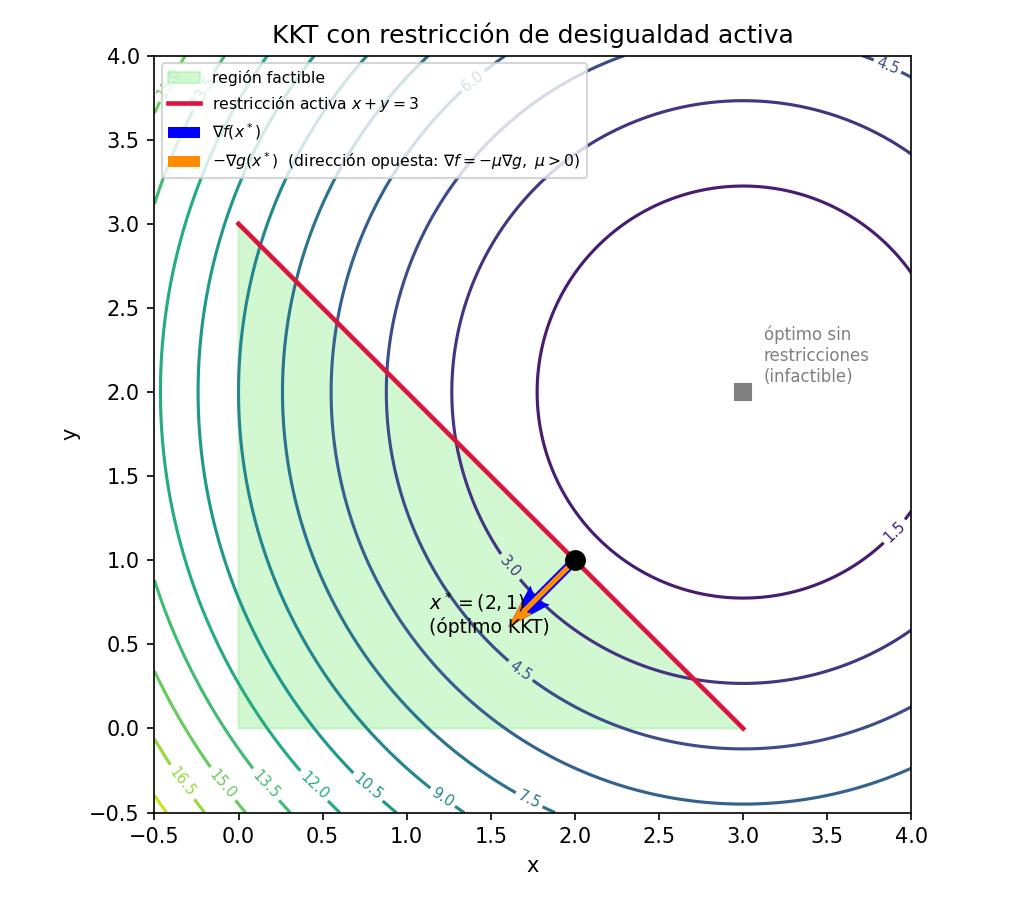
\includegraphics[height=3.8cm,keepaspectratio]{fig11_kkt_desigualdad.png}
  \end{center}
\end{frame}

\begin{frame}[fragile]{KKT en Python (con \texttt{scipy.optimize})}
\begin{lstlisting}
from scipy.optimize import minimize

f = lambda v: (v[0]-3)**2 + (v[1]-2)**2
restricciones = [
    {"type": "ineq", "fun": lambda v: 3 - v[0] - v[1]},  # x+y<=3
    {"type": "ineq", "fun": lambda v: v[0]},              # x>=0
    {"type": "ineq", "fun": lambda v: v[1]},              # y>=0
]
sol = minimize(f, x0=[0, 0], constraints=restricciones)
print(sol.x)     # ~ [2. 1.]
\end{lstlisting}
  \small Script completo (versión gráfica):
  \texttt{scripts/11\_kkt\_desigualdad.py}
\end{frame}

% ==================================================================
\section{Síntesis de la clase}
% ==================================================================

\begin{frame}{Mapa de conceptos}
  \small
  \begin{center}
  \begin{tabular}{ll}
    \toprule
    \textbf{Concepto} & \textbf{Para qué sirve en optimización} \\
    \midrule
    Derivada / parcial & Medir razón de cambio \\
    Gradiente $\grad f$ & Generaliza la derivada; dirección de máx.\ cambio \\
    Curvas de nivel & Visualizar $f$; $\grad f \perp$ curva de nivel \\
    Derivada direccional & Cambio de $f$ en cualquier dirección \\
    Puntos críticos & Candidatos a óptimo ($\grad f=\mathbf 0$) \\
    Hessiana & Clasifica puntos críticos (mín / máx / silla) \\
    Serie de Taylor & Modelo cuadrático local (base de métodos tipo Newton) \\
    Convexidad & Garantiza que mínimo local = mínimo global \\
    Lagrange & Óptimo con restricciones de igualdad \\
    KKT & Óptimo con restricciones de igualdad y desigualdad \\
    \bottomrule
  \end{tabular}
  \end{center}
\end{frame}

\begin{frame}{Fórmulas clave (resumen)}
  \small
  \begin{align*}
    \text{Gradiente:} \quad & \grad f(\x) = \left(\partial f/\partial x_1,\dots,\partial f/\partial x_n\right) \\
    \text{Derivada direccional:} \quad & D_\u f(\x) = \grad f(\x)\cdot \u \\
    \text{Taylor orden 2:} \quad & f(\x_0+\dd)\approx f(\x_0)+\grad f(\x_0)^\top\dd+\tfrac12\dd^\top \Hess(\x_0)\dd \\
    \text{Convexidad (1er orden):} \quad & f(\mathbf y)\ge f(\x)+\grad f(\x)^\top(\mathbf y - \x) \\
    \text{Punto crítico:} \quad & \grad f(\x^*)=\mathbf 0 \\
    \text{Lagrange:} \quad & \grad f(\x^*)=\lambda\grad h(\x^*),\ h(\x^*)=0 \\
    \text{KKT (estacionariedad):} \quad & \grad f(\x^*)+\mu^*\grad g(\x^*)=\mathbf 0,\ \mu^*\ge0,\ \mu^* g(\x^*)=0
  \end{align*}
\end{frame}

\begin{frame}{¿Qué sigue en el curso?}
  Con este lenguaje matemático ya podemos estudiar \textbf{métodos}
  concretos de optimización:
  \begin{itemize}
    \item \textbf{Clase 2:} Métodos de descenso de gradiente (tasa de
      aprendizaje, convergencia, casos convexos vs.\ no convexos).
    \item \textbf{Clase 3:} Método de Newton y cuasi-Newton (uso del
      modelo cuadrático de Taylor).
    \item \textbf{Clase 4:} Programación lineal (simplex, dualidad).
    \item \textbf{Clase 5:} Programación no lineal con restricciones,
      KKT en profundidad, penalización y barrera.
    \item \textbf{Clases posteriores:} optimización estocástica,
      metaheurísticas, aplicaciones.
  \end{itemize}
\end{frame}

% ==================================================================
\section{Ejercicios propuestos}
% ==================================================================

\begin{frame}{Ejercicios para la próxima clase}
  \small
  \begin{enumerate}
    \item Calcule $\grad f$ y los puntos críticos de $f(x,y)=x^3-3xy+y^3$;
      clasifíquelos con la Hessiana.
    \item Muestre, usando la definición de la cuerda, que $f(x)=e^x$ es
      convexa. Verifíquelo también con $f''(x)$.
    \item Encuentre la dirección de máximo ascenso de
      $f(x,y)=\ln(x^2+y^2+1)$ en el punto $(1,2)$.
    \item Resuelva con multiplicadores de Lagrange: maximizar
      $f(x,y)=xy$ sujeto a $x+y=10$. Interprete $\lambda$.
    \item Plantee las condiciones KKT para
      $\min (x-1)^2+(y-1)^2$ s.a.\ $x^2+y^2\le 1$, y resuélvalas a mano.
    \item \textbf{Código:} modifique \texttt{scripts/09\_min\_local\_global.py}
      para $f(x)=x^4-5x^2+4$ y reporte todos los mínimos/máximos locales
      y cuál es global.
    \item \textbf{Código:} modifique \texttt{scripts/03\_curvas\_nivel\_gradiente.py}
      para $f(x,y)=\sin(x)\cos(y)$ y comente qué observa en el campo
      gradiente cerca de los puntos de silla.
  \end{enumerate}
\end{frame}

% ==================================================================
\section{Referencias}
% ==================================================================

\begin{frame}{Referencias}
  \footnotesize
  \begin{itemize}
    \item S. Boyd, L. Vandenberghe. \emph{Convex Optimization}. Cambridge
      University Press, 2004. (Disponible gratis en línea.)
    \item J. Nocedal, S. Wright. \emph{Numerical Optimization}, 2.\textsuperscript{a}
      ed. Springer, 2006.
    \item D. Bertsekas. \emph{Nonlinear Programming}, 3.\textsuperscript{a}
      ed. Athena Scientific, 2016.
    \item J. Stewart. \emph{Cálculo de varias variables: trascendentes
      tempranas}. Cengage Learning.
    \item T. Apostol. \emph{Calculus}, Vol.\ 2. Wiley.
    \item Documentación de \texttt{NumPy}, \texttt{SciPy} y
      \texttt{Matplotlib}: \url{https://numpy.org},
      \url{https://scipy.org}, \url{https://matplotlib.org}.
  \end{itemize}
\end{frame}

\begin{frame}[standout]
  ¿Preguntas?
\end{frame}

\end{document}
